\documentclass[problem]{mcs}

\begin{pcomments}
  \pcomment{PS_koch_induction_triangle}
  \pcomment{variation of PS_koch_induction, but with simpler algebra}
  \pcomment{CH, 4/10/14}
\end{pcomments}

\pkeywords{
  induction
  equilateral
  recurrence
  geometric
  sum
}

%%%%%%%%%%%%%%%%%%%%%%%%%%%%%%%%%%%%%%%%%%%%%%%%%%%%%%%%%%%%%%%%%%%%%
% Problem starts here
%%%%%%%%%%%%%%%%%%%%%%%%%%%%%%%%%%%%%%%%%%%%%%%%%%%%%%%%%%%%%%%%%%%%%

\begin{problem}
Here is an interesting construction of a geometric object known as the
\emph{Koch snowflake}.  Define a sequence of polygons $S_0, S_1$
recursively, starting with $S_0$ equal to an equilateral triangle with
unit sides.  We construct $S_{n+1}$ by removing the middle third of
each edge of $S_n$ and replacing it with two line segments of the same
length, as illustrated in Figure~\ref{kochind}.

\begin{figure}[h]
  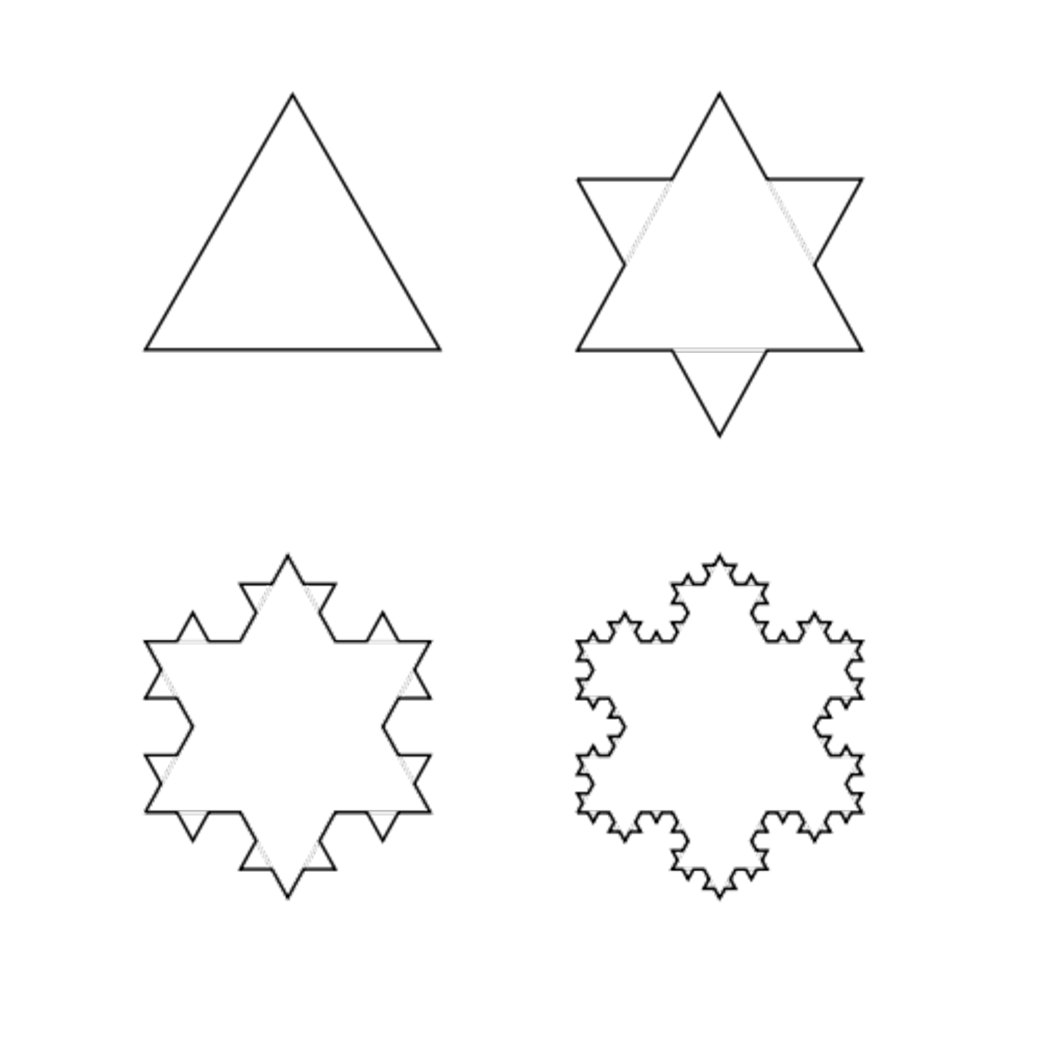
\includegraphics[width=2.5in]{koch_full}
  \caption{$S_0,S_1,S_2 \text{ and } S_3$.}
  \label{kochind}
\end{figure}

Let $a_n$ be the area of $S_n$.  Observe that $a_0$ is just the area
of the unit equilateral triangle which by elementary geometry is
$\sqrt{3}/4$.

Prove by induction that for $n \geq 0$, the area of the $n^{\text{th}}$
 snowflake is given by:
\begin{equation}\label{an1s3}
  a_n = a_0 \paren{\frac{8}{5} - \frac{3}{5} \paren{\frac{4}{9}}^n}.
\end{equation}

\begin{staffnotes}
\hint  If need be, prompt for the recurrence~\eqref{an+1a}.
\end{staffnotes}


\begin{solution}
Let $l_n$ be the length of the edges in $S_n$, and $e_n$ be the number
of edges in $S_n$.  So, $l_0=1$, and $e_0=3$.  From the definition of
$S_{n+1}$, we have
\begin{align}
l_{n+1} & = l_n/3,\label{ln+13}\\
e_{n+1} & = 4e_n,\label{en+14}\\
a_{n+1} & = a_n + e_n \cdot a_0 \paren{l_{n+1}}^2.\label{an+1a}
\end{align}
The last equation arises since the area of an equilateral triangle
with edge length $l$ is $a_0 l^2$.

Clearly,
\begin{equation}
l_n = (1/3)^{n} \qquad \text{and}\qquad e_n = 3 \cdot 4^{n},
\end{equation}
as can be verified by a trivial induction.

We now use~\eqref{an+1a} to prove by induction on $n$
that~\eqref{an1s3} holds for all $n \geq 1$, with~\eqref{an1s3}
serving as Induction Hypothesis.

\begin{proof}
\inductioncase{Base case}: ($n=0$).  The right hand side
of~\eqref{an1s3} simplifies to $a_0$ when $n=0$.

\inductioncase{Induction step}: Assume the Induction Hypothesis is
true for some positive integer $m$.  That is,
\begin{equation}\label{85indhyp}
 a_m =  a_0 \paren{\frac{8}{5} - \frac{3}{5} \paren{\frac{4}{9}}^m} .
\end{equation}
From~\eqref{an+1a}, we have:
\begin{align*}
a_{m+1} & = a_m + e_m \cdot a_0 \cdot \paren{l_{m+1}}^2 \\
      & = a_m + 3 \cdot 4^{m} \cdot a_0 \cdot \paren{(1/3)^{m+1}}^2 \\
      & = a_m + a_0  \cdot 3 \cdot 4^{m} (1/9)^{m+1} \\
      & = a_m + a_0 \cdot 3 (1/9) \cdot \paren{\frac{4}{9}}^{m}\\
      & = a_0 \paren{\frac{8}{5} - \frac{3}{5} \paren{\frac{4}{9}}^m}
      + a_0 \cdot \frac{1}{3} \cdot \paren{\frac{4}{9}}^{m} & \text{(by induction hypothesis~\eqref{85indhyp})}\\
      & = a_0 \paren{\frac{8}{5} +
                \paren{\frac{1}{3}  - \frac{3}{5}}  \paren{\frac{4}{9}}^{m}}\\
      & = a_0 \paren{\frac{8}{5} -
                \paren{\frac{4}{3 \cdot 5}} \paren{\frac{9}{4}} \paren{\frac{4}{9}}^{m+1}}\\
      & = a_0 \paren{\frac{8}{5} - \frac{3}{5} \paren{\frac{4}{9}}^{m+1}}
\end{align*}
which proves the Induction Hypothesis for $n = m+1$. 

\end{proof}

\begin{staffnotes}
By the way, we derived~\eqref{an1s3} using the formula for a geometric sum:
 \begin{align*}
 a_n & =  a_{n-1} + 3\cdot 4^{n-1} \cdot a_0 (1/9)^n\\
     & =  a_{n-1} + 3 a_0 (1/9) \paren{\frac{4}{9}}^{n-1}\\
     & = a_0 + 3a_0 (1/9) \sum_{k=0}^{n-1} \paren{\frac{4}{9}}^k\\
     & = a_0 \paren{1 + (1/3)\frac{1- (4/9)^n}{1-4/9}}\\
     & = a_0 \paren{1 + (1/3)\frac{1- (4/9)^n}{5/9}}\\
     & = a_0 \paren{\frac{8}{5} - \frac{3}{5}\paren{\frac{4}{9}}^n}
 \end{align*}
\end{staffnotes}

So as $n$ goes to infinity, the area $a_n$ approaches $8/ 5$ while the
perimeter approaches a nowhere differentiable curve whose length is
$\lim_{n \to \infty} e_n l_n = \lim_{n \to \infty} 3 \cdot (4/3)^n =
\infty$.

\end{solution}

\end{problem}

%%%%%%%%%%%%%%%%%%%%%%%%%%%%%%%%%%%%%%%%%%%%%%%%%%%%%%%%%%%%%%%%%%%%%
% Problem ends here
%%%%%%%%%%%%%%%%%%%%%%%%%%%%%%%%%%%%%%%%%%%%%%%%%%%%%%%%%%%%%%%%%%%%%

\endinput

